\documentclass[a4paper, 12pt]{article}
\usepackage[top=1in, right=1in, bottom=1in, left=1.25in]{geometry}
\usepackage{xcolor}
\usepackage{graphicx}
\usepackage{float}


\begin{document}
    \section{SYSTEM DESCRIPTION}
    The Hotel Management System is designed to manage guest reservation, room inventory, payment processing, service order, staff administration, and facility maintenance through an integrated relational database. It provides centralized data management for all hotel activities for all hotel activities, ensuring operational efficiency, accurate financial tracking and enhanced guest satisfaction.

    \subsection{Core Entities}
    \begin{enumerate}
        \item \textbf{Guest:} 
                Stores customer informations including GuestID as unique identifier, name, email, phone and date of birth. It maintains complete guest profiles for personalized service, booking, history and analytics.
        \item \textbf{Booking:}
                Represents hotel reservation attribute for BookingID, booking date, number of guest, total amount and status of booking. It served ad central entity linking guests, rooms, payment and services. Each booking is made my exactly one guest but can include multiple rooms.
        \item \textbf{Room:}
                Manages hotel inventory with RoomID, room type (Standard, Deluxe or Suite), floor number, base price and status. It tracks availibility and enables dynamic pricing based on demand.
        \item \textbf{Payment:}
                Records financial transaction with PaymentID, amount, paymenr date, status, and payment method (cash, card or online transfer). It supports multiple payment per booking for deposits.
        \item \textbf{Service:}
                Define the additional amenities including ServiceID, name, type, base charge and description of the service. It represent revenue streams beyond the booked room price.
        \item \textbf{Service\_Order:}
                Tracks the individual service requests with the OrderID, order timestamp, quantity (if applies), amount and status. It links the booking to service with order-specific details. It is weak entity and cannot exist withot a booking.
        \item \textbf{Staff:}
                Contains employee information including StaffID, name, email, phone, hire date and salary. Each staff is assigned to one department and holds single primary role.
        \item \textbf{Department: }
                Organized staffs into functional units with the DeptID, department name and also ManagerID (foreign key referencing to the staff). Each department has one manager.
        \item \textbf{Role:}
                Defines job position with RoleID, name, and base salary. It establishes salary range and system access permissions.
        \item \textbf{Maintenance\_Request:}
                Tracks facility maintenance with RequestID, request date, issue description, priority and status. It links maintenance issue to specific rooms and assigned staff.
    \end{enumerate}

    \newpage

    \subsection{Key Relationships}
    \begin{enumerate}
        \item \textbf{Makes (Guest - Booking) }\\
                \textit{One-to-Many}: Each guest can make multiple booking over time, but each booking can belong to exactly one guest.
        \item \textbf{Reserves (Booking - Room)}\\
                \textit{Many-to-Many}: Bookings can reserve  multiple room (group booking), and rooms can be reserved by different booking over time. It includes check-in date, check-out date and room price attribute.
        \item \textbf{Settles (Booking - Payment)}\\
                \textit{One-to-Many}: One booking can have multiple payments, but each payment can belong to single booking. 
        \item \textbf{Orders (Booking - Service via Service\_Order)}\\
                \textit{Many-to-Many}: Guests can order multiple service during stay through ServiceOrder entiry. Service charges are added to final booking bill.
        \item \textbf{WorksIn (Staff - Department)}\\
                \textit{Many-to-One}: Each staff member works in exactly department but a department can have multiple staffs.
        \item \textbf{HasRole (Staff - Role)}\\
                \textit{Many-to-One}: Each staff member had one primary role but a specific role can have multiple staffs (for eg, a person can be cook but kitchen can have multiple cooking staff).
        \item \textbf{Reported\_For (Maintenance\_Request - Room)}\\
                \textit{Many-to-One}: Each maintenance request is for one room, but rooms can have multiple requests over time. 
        \item \textbf{Assigned\_To (Maintenance\_Request - Staff)}\\
                \textit{Many-to-One}: Each request is assigned to one staff memmber.
    \end{enumerate}
    \newpage
    \section{ENTITY RELATION (ER) DIAGRAM}
    \begin{figure}[H]
        \centering
            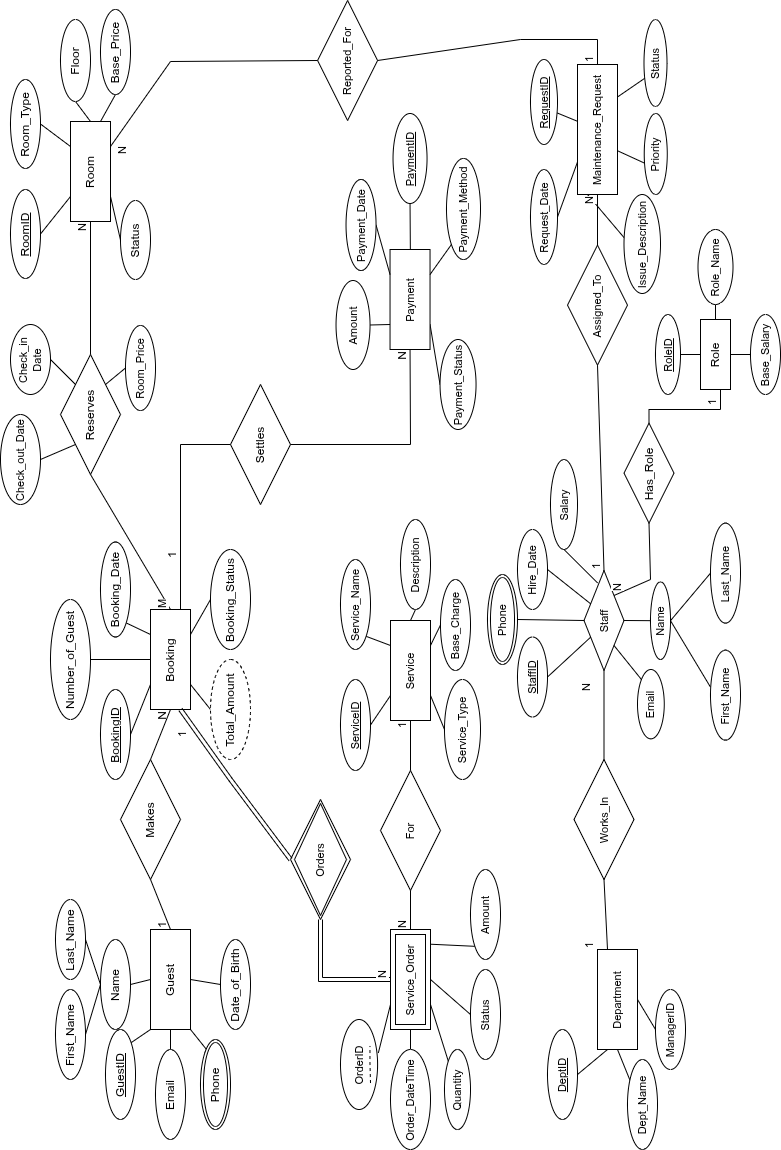
\includegraphics[width=\textwidth]{Hotel Management ER.png} 
            \caption{Hotel Management ER Diagram}         
    \end{figure}
\end{document}


